\chapter{notes 1}\label{n1}

Numerical modelling, sedimentary sequence interpretation suggest cyclical periods of ice-sheet expansion and retreat\cite{Young2011}. 
use ice-penetrating radar data to generate a new basal bed topography of the Aurora Subglacial Basin (ASB) in east Antarctica is characterised by a fjord landscape (this land is under $\sim$ under $2-4.5$ km of ice). The ASB has a potentially significant influence on the east Antarctic ice-sheet (EAIS), however there is high uncertainty in estimates of past and present global sea level changes due to the scarcity of bed data\cite{Young2011}. This uncertainty also limits the accuracy of models used to predict future ice sheet growth or decay

\begin{Figure}
\centering
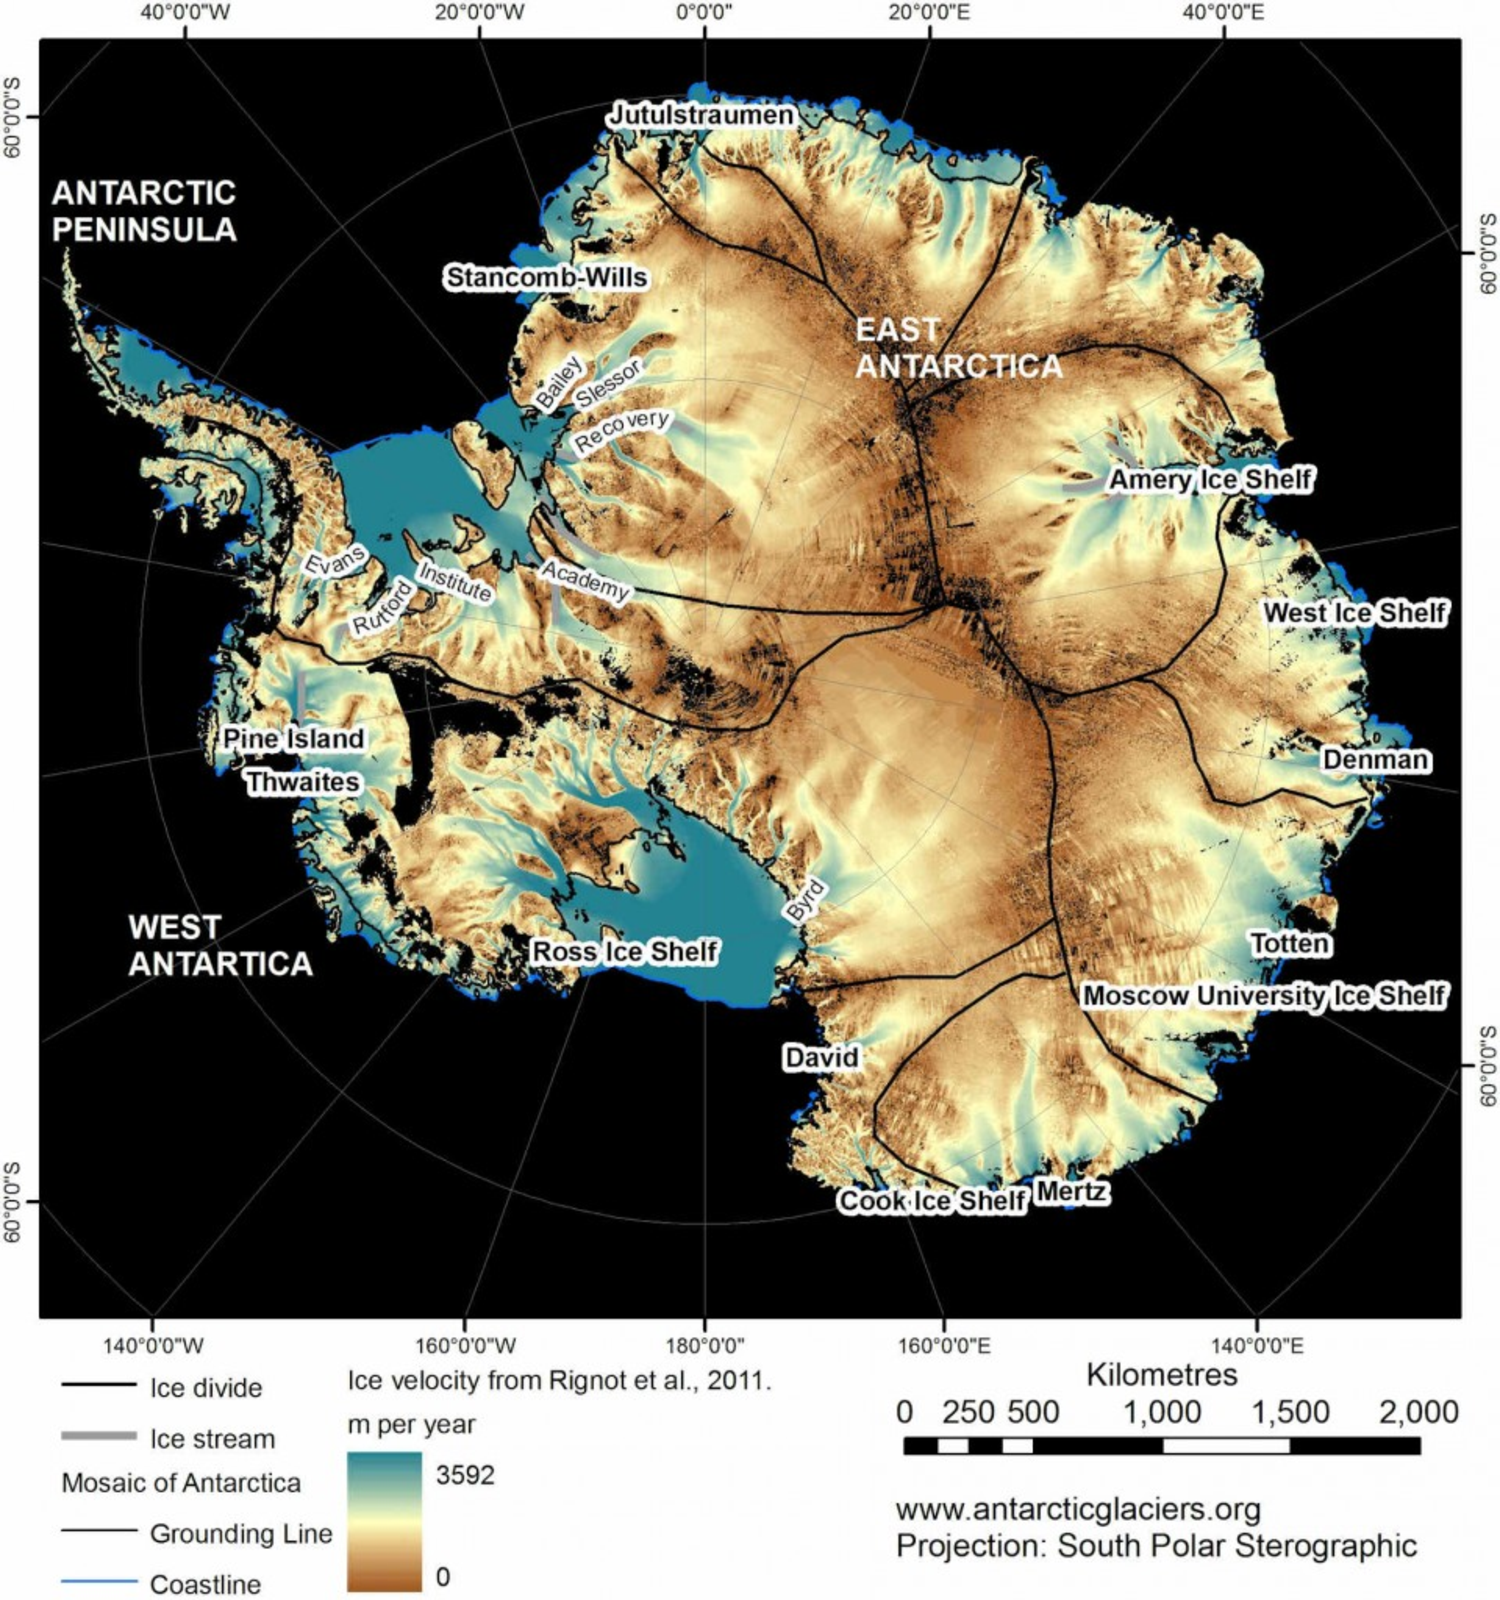
\includegraphics[width=\linewidth]{antarctica_velocity.pdf}
\captionof{figure}{}
\label{fig:Antarctica_velocity}
\end{Figure}

Unknown terms
{\small \begin{itemize}
\item{Channel incision}
\item{Alpine style glaciation}
\end{itemize}
}

TOOLS
{\small \begin{itemize}
\item{ICECAP aero geophysical programme}
\item{BEDMAP}
\end{itemize}
}

MATHS
{\small \begin{itemize}
\item{Lagrangian interpolation}
\item{natural-neighbour interpolation}
\end{itemize}
}
